\documentclass{article}

% formato
\usepackage[margin = 1.5cm, letterpaper]{geometry}
\usepackage[utf8]{inputenc}

% autómatas
\usepackage{tikz}
\usetikzlibrary{automata, positioning}

%formato ecuaciones
\usepackage{amsmath}

% símbolos
\usepackage{amssymb}

% manejo de tablas
\usepackage{float}

\begin{document}
    \title{
        Autómatas y Lenguajes formales \\
        Ejercicio Semanal 6
    }

    \author{
        Sandra del Mar Soto Corderi \\
        Edgar Quiroz Castañeda
    }

    \date{
        14 de marzo del 2019
    }
    
    \maketitle

    \begin{enumerate}
        \item {
            Para cada 	$ANF_{\epsilon}$, resuelve los siguientes incisos.
            \begin{enumerate}
                \item Calcula la $\epsilon$-cerradura de cada estado.\\
                
                \item Elimina las $\epsilon$-transiciones obteniendo un AFN, mostrando el proceso de cálculo de las nuevas transiciones.\\
            \end{enumerate}
        }
       \end{enumerate}
    	\begin{enumerate}
    		\item {
    			Autómata 1
    			\begin{figure} [H]
    				\centering
    				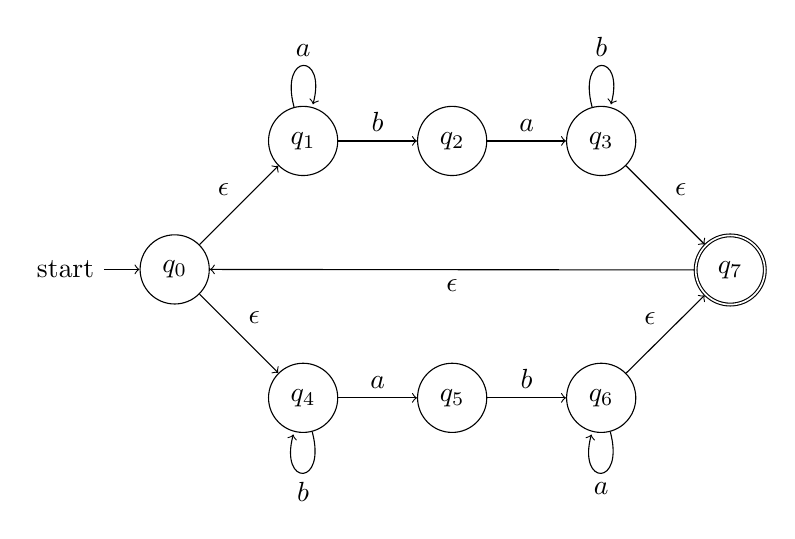
\begin{tikzpicture}[auto]
    				% estados
    				\node [state, initial] (q0) {$q_{0}$};
    				\node [state] (q1) [above right=of q0] {$q_{1}$};
    				\node [state] (q2) [right=of q1] {$q_{2}$};
    				\node [state] (q3) [right=of q2] {$q_{3}$};
    				\node [state] (q4) [below right=of q0] {$q_{4}$};
    				\node [state] (q5) [right=of q4] {$q_{5}$};
    				\node [state] (q6) [right=of q5] {$q_{6}$};
    				\node [state, accepting] (q7) [below right=of q3] {$q_{7}$};
    				
    				% transiciones
    				\path[->]
    				(q0) edge node {$\epsilon$} (q1)
    				(q0) edge node {$\epsilon$} (q4)
    				(q1) edge [loop above] node {$a$} (q1)
    				(q3) edge [loop above] node {$b$} (q3)
    				(q4) edge [loop below] node {$b$} (q4)
    				(q6) edge [loop below] node {$a$} (q6)
    				(q3) edge node {$\epsilon$} (q7)
    				(q6) edge node {$\epsilon$} (q7)
    				(q7) edge node {$\epsilon$} (q0)
    				(q1) edge node {$b$} (q2)
    				(q2) edge node {$a$} (q3)
    				(q4) edge node {$a$} (q5)
    				(q5) edge node {$b$} (q6);
    				\end{tikzpicture}
    			\end{figure}
    		}
    	\item {
    		Autómata 2
    		\begin{figure} [H]
    			\centering
    			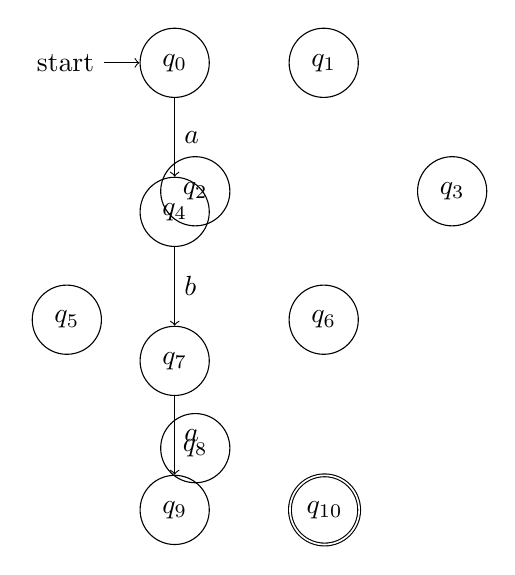
\begin{tikzpicture}[auto]
    			% estados
    			\node [state, initial] (q0) {$q_{0}$};
    			\node [state] (q1) [right=of q0] {$q_{1}$};
    			\node [state] (q2) [below left=of q1] {$q_{2}$};
    			\node [state] (q3) [below right=of q1] {$q_{3}$};
    			\node [state] (q4) [below=of q0] {$q_{4}$};
    			\node [state] (q5) [below left=of q2] {$q_{5}$};
    			\node [state] (q6) [below right=of q2] {$q_{6}$};
    			\node [state] (q7) [below=of q4] {$q_{7}$};
    			\node [state] (q8) [below left=of q6] {$q_{8}$};
    			\node [state] (q9) [below=of q7] {$q_{9}$};
    			\node [state, accepting] (q10) [right=of q9] {$q_{10}$};
    			
    			% transiciones
    			\path[->]
    			(q0) edge node {$a$} (q4)
    			(q4) edge node {$b$} (q7)
    			(q7) edge node {$a$} (q9)
    		
;
    			\end{tikzpicture}
    		\end{figure}
    	}
    
    \end{enumerate}
\end{document}